\clearpage
\section*{Supplementary Information}

This Supplementary Information expands the main-text Methods and Results. It documents the evidence architecture, cohort contracts, model implementation, leakage controls, statistical plan, locked confirmation, routing exploration and extension analyses in RADCURE, TCGA-HNSC and GEO. All numerical summaries are derived from frozen aggregate artifacts; no patient-level predictions are included.

\setcounter{figure}{0}
\setcounter{table}{0}
\renewcommand{\thefigure}{S\arabic{figure}}
\renewcommand{\thetable}{S\arabic{table}}
\setlength{\LTcapwidth}{\textwidth}
\renewcommand{\arraystretch}{1.08}

\section*{S1~Evidence architecture and claim map}
The study was organized as a staged evidence pipeline. Repeated nested cross-fitting in the HANCOCK development cohort quantified the incremental value of the V1R residual pathway over a clinical-pathological anchor. A monotone calibration bridge was then optimized and evaluated within development folds. Raw V1R predictions and all analysis dependencies were sealed before confirmation outcomes were accessed. Finally, router, RADCURE, transcriptome and GEO analyses examined selective use, contemporary benchmarking, method transfer and platform transport.

This architecture separates four claims. First, V1R showed a reproducible development gain, favourable in all five repetition seeds, with complete coverage and pattern-level safety within the prespecified boundary. Second, the HANCOCK confirmation cohort showed favourable point estimates for every principal metric; the bootstrap intervals reflected the moderate event count and supported a consistent directional signal. Third, the development bridge improved calibration summaries, whereas the later bridge readout identified cohort-level probability recalibration as the next step for transportable absolute-risk output. Fourth, router and extension analyses provide design insight and transport evidence complementary to the locked raw-V1R result.

This separation is a strength of the study. Model development, calibration, confirmation and extension are distinguished by frozen protocols and explicit artifact boundaries. The central finding---controlled incremental multimodal evidence can improve risk ranking while preserving full output availability---can therefore be evaluated alongside calibration, routing and transport considerations without conflating exploratory signals with locked confirmation.

\section*{S2~HANCOCK cohorts, prediction time and endpoint}
HANCOCK was the primary development and confirmation ecosystem. The development analysis included 610 eligible postoperative patients with 173 deaths; the locked confirmation analysis included 152 patients with 40 events. Of 763 source records, one was excluded and 762 eligible postoperative patients remained. The split preserved a separately sealed outcome cohort while retaining sufficient development events for repeated nested cross-fitting.

For patient $i$, $T_i$ denotes event time, $C_i$ censoring time, $Y_i=\min(T_i,C_i)$ observed duration and $\delta_i=I(T_i\le C_i)$ the event indicator. Follow-up began at first treatment and ended at last information; the event was all-cause death. Non-positive durations were excluded. The primary horizon was $t^*=730.5$ days, approximately 24 months. The intended prediction time was immediately after definitive surgery and pathological review, using information available at that point and excluding post-prediction outcome information.

The clinical anchor used age, sex, smoking, primary site, grade, p16, resection, pathological T category and pathological N category. Optional blood, ICD-coded comorbidity and tissue-microarray inputs were admitted only through the residual pathway. This ordering mirrors clinical deployment: the anchor contains routinely available postoperative variables, whereas optional modalities may differ in completeness and preprocessing success.

\section*{S3~Acquisition, usability and quality contract}
For optional modality $m$, the contract distinguished acquisition $a_{im}$, usability $u_{im}$ and an outcome-blind quality vector $q_{im}$. Acquisition indicated that a source record or assay existed. Usability indicated that the frozen preprocessing contract could produce a valid model input. The usable set was
\begin{equation}
\mathcal{M}_i=\{m:u_{im}=1\}.
\end{equation}

Quality summaries included missing fraction, out-of-range counts, assay completeness and distributional distance from training data. Absent and acquired-but-unusable measurements were represented structurally rather than as zero-valued biology. The natural acquisition pattern was the blood--ICD--TMA usability tuple. Pattern counts and quality distributions were computed without outcomes. For development safety analyses, a supported pattern required at least 30 patients and 10 events; rarer patterns were descriptive and did not receive pattern-specific tuning.

Of 762 eligible patients, 693 blood, 712 ICD and 736 tissue-microarray records were acquired, whereas 683, 712 and 736, respectively, were usable. Thus, ten acquired blood records failed the usability contract. Complete blood and TMA records numbered 604 and 639; 79 blood and 97 TMA records were partially usable. This contract preserves the distinction between absence, partial usability and acquired-but-unusable evidence.

The clinical-pathological anchor was fixed to age at diagnosis, sex, smoking status, primary tumour site, grade, p16 association, resection status, pathological T category and pathological N category. Pathology belonged to the postoperative anchor rather than being treated as an optional token. Adjuvant treatment, recurrence, progression, metastasis recorded after the prediction time and outcome-derived variables were prohibited predictors. Optional blocks remained separate at the data boundary; they were not concatenated into a complete-case matrix before availability and usability had been assigned.

The blood block used a fixed panel of 16 haematology measurements from the prespecified pre-treatment window. A missing blood row denoted non-acquisition, whereas a present row with invalid or entirely missing measurements could be acquired but unusable. Partially observed usable rows retained within-block missingness for fold-bound imputation and explicit missingness indicators. TMA followed the same structural rule: absence of a row represented modality absence; missing values within an existing row represented within-modality incompleteness. This distinction prevented biological zeros from being substituted for unavailable assays.

The locally available ICD block consisted of 40 pre-extracted code groups. The underlying vocabulary had been generated with a corpus-level minimum document frequency of three, and the raw text source was not available for reconstruction. ICD was therefore marked as having conditional provenance. It was retained in the frozen evidence contract, but this limitation is disclosed because a fully fold-pure vocabulary sensitivity analysis would be preferable in a future release.

Separate fold-bound preprocessors handled the clinical mixed-type block and the three numeric optional blocks. Training-fold medians, scaling parameters, categorical levels and one-hot mappings were estimated only from explicitly allowed fit identifiers. New categories at transform time mapped to an unknown level. The preprocessing interface rejected held-out identifiers during fitting and returned missingness indicators alongside transformed values. These checks made leakage control executable rather than dependent only on analyst convention.

\section*{S4~Clinical anchor and residual network}
The V0 anchor was an elastic-net Cox proportional-hazards model \cite{cox1972,breslow1974}. After training-fold preprocessing,
\begin{equation}
\eta_{\mathrm{V0},i}=x_{c,i}^{\mathsf T}\hat\beta_c.
\end{equation}
Encoding, imputation, scaling and category handling were confined to the corresponding training fold. A training-fold Breslow baseline-hazard estimator converted the linear predictor to 24-month mortality risk.

V1R was a clinically anchored residual Deep Sets Cox backbone with 3,225 parameters. Each usable modality was represented as an unordered token containing its measurements, learned representation, modality identity, usability status and quality indicators:
\begin{equation}
h_i=\rho\left(\frac{1}{|\mathcal{M}_i|}\sum_{m\in\mathcal{M}_i}\phi(x_{im},q_{im},e_m)\right),\qquad
\Delta\eta_{\mathrm{res},i}=g(h_i).
\end{equation}
The fused score was
\begin{equation}
\eta_{\mathrm{V1R},i}=\eta_{\mathrm{V0},i}+\lambda_f\Delta\eta_{\mathrm{res},i}.
\end{equation}
The token form makes the input set permutation invariant, while the masked mean allows any non-empty usable subset to be processed. When $\mathcal{M}_i$ is empty, the residual and fused-score deviations are exactly zero, so V1R returns V0 deterministically.

\section*{S5~Nested cross-fitting, optimization and leakage control}
Repeated nested cross-fitting used five outer folds, three inner folds and repetition seeds 17, 29, 43, 71 and 101. Preprocessing, feature selection where applicable, model fitting, shrinkage selection and baseline-hazard estimation were confined to training folds. For each outer fold $f$, inner cross-validation searched residual penalties $\{0.01,0.1,1.0\}$, optimization checkpoints $\{0,10,25,50\}$ and residual scales $\{0.1,0.2,0.3,0.4,0.5,1.0\}$.

This design yields 25 matched V0/V1R members (five seeds by five outer folds) and supports paired fold-level and seed-level summaries. Outer-fold outcomes were not used for hyperparameter selection. Repeated out-of-fold rows provided the development performance estimates and the calibration-bridge diagnostic, while seed-level paired differences assessed reproducibility. No confirmation outcomes entered development tuning.

The V1R stage was a transparently result-informed rescue of the original unscaled V1 analysis. The original U2 decision, \texttt{V1\_DOES\_NOT\_EARN\_COMPLEXITY}, remains unchanged. Prediction-space sensitivity analysis indicated that the unscaled residual was too aggressive; scales near 0.2--0.4 reduced pattern regret and calibration-slope deterioration while retaining a small, seed-stable discrimination signal. V1R therefore added residual scale to the inner-loop search and was labelled post-hoc exploratory rather than retrospectively reclassifying the original V1 result.

The frozen V1R selection objective minimized mean inner-fold IPCW Brier score at 730.5 days, with mean inner-fold Uno C as the secondary criterion. Deterministic ties favoured the larger residual penalty, then the smaller residual scale, then fewer optimization steps. Architecture search and broad hyperparameter sweeps were prohibited. The implementation used deterministic PyTorch computation on CPU in float64, Adam optimization with learning rate 0.003, weight decay 0.0001 and gradient clipping at norm 5.0. The loss combined mean negative Breslow partial likelihood with an L2 penalty on the residual score.

After the inner-loop candidate was selected, the corresponding outer-training fold was refitted and its Breslow baseline hazard was estimated after residual scaling using training outcomes only. Each patient was predicted exactly once per repetition. Patient-level out-of-fold predictions were stored outside tracked manuscript artifacts; only aggregate audits and frozen specifications were committed. The rescue gate retained the original safety thresholds and could authorize only a development signal, not confirmatory superiority or external validation.

\section*{S6~Global calibration bridge}
The U5R7 bridge was frozen as \texttt{beta\_0.900\_logloss}. For raw V1R 24-month risk $p_{\mathrm{V1R}}$ in held-out outer fold $f$,
\begin{align}
x_{\mathrm{raw},i}&=\operatorname{logit}(p_{\mathrm{V1R},i}),\\
x_{\mathrm{bridge},i}&=\alpha_{\mathrm{logloss},f}+0.90x_{\mathrm{raw},i},\qquad
p_{\mathrm{bridge},i}=\sigma(x_{\mathrm{bridge},i}).
\end{align}
The intercept was fitted by weighted log-loss using only non-held-out development folds. The bridge was global and pattern-agnostic, with a fixed positive slope. It was therefore strictly monotone, preserved ranking, retained 100\% coverage and did not alter the exact V0 fallback.

The diagnostic population contained 2,460 repeated out-of-fold rows and 415 evaluable events. Gates were global Brier change $\le +0.0005$, worst supported-pattern regret $\le +0.005$, improved calibration-in-the-large and calibration slope, ranking preservation and full coverage. Confirmation outcomes were not used for fitting or tuning.

U5R7 followed a sequence of development-only bridge explorations and froze the candidate identifier \texttt{beta\_0.900\_logloss} before its diagnostic readout. The positive slope was not estimated separately by pattern, and the intercept was fitted anew within each non-held-out development partition. Thus, the bridge could move the absolute probability scale without changing within-fold ordering. It also left the raw V1R score, V0 anchor, acquisition rules and empty-set fallback untouched.

The bridge diagnostic is not numerically interchangeable with the primary development table. It contains repeated evaluable out-of-fold rows and addresses whether a global monotone transformation improves absolute-risk calibration; the primary table compares V0 and raw V1R as prediction models. The small positive Brier change was retained in the report rather than hidden. U5R7 passed its prespecified development-safe gates, but the decision authorized only a development calibration candidate. Raw V1R remained the primary prediction path and the only fused model carried into the locked confirmation comparison.

\section*{S7~Locked confirmation and secondary bridge protocol}
The confirmation protocol, input manifest, dependency lock and prediction artifact were frozen before confirmation outcomes were unsealed. Twenty-five matched V0/V1R members were generated using five seeds and five outer folds, with development-fold fitting only and no confirmation tuning, bridge, router, refitting or selective patient removal. Outcomes were read after prediction sealing.

Aggregate uncertainty used 2,000 patient-level stratified bootstrap replicates (seed 20260825). The primary confirmation readout was raw V1R. U5R8 separately reused the frozen $\beta=0.90$ bridge with the arithmetic mean development intercept $\alpha=-0.1450338$, using 2,000 event-stratified replicates (seed 20260827). Because U5R8 occurred after raw-outcome unsealing, it is reported as a locked secondary post-unseal validation and is interpreted as evidence about probability-scale transport rather than ranking.

The locking sequence separated prediction generation from outcome evaluation. The sealed input manifest identified the eligible confirmation records and the exact source variables consumed by V0 and V1R. The dependency receipt fixed the execution environment, and the prediction receipt recorded the patient-level artifact before the event file was joined. Aggregate metrics were then computed from the sealed predictions. The confirmation cohort therefore supplied no information for preprocessing, hyperparameter choice, residual shrinkage, baseline-hazard estimation, threshold selection or model refitting.

The 25 members were kept matched between V0 and V1R so that every paired contrast compared predictions obtained under the same repetition and outer-fold training role. Coverage was evaluated before performance summaries and remained 100\% for both models. Bootstrap sampling operated on patients rather than the 25 repeated prediction rows; this preserved within-patient dependence and prevented artificial precision from treating repeated predictions as independent observations. The bridge was excluded from the primary confirmation estimand because it had been developed as a separate calibration layer. Its later reuse in U5R8 did not modify the locked raw-V1R result.

\section*{S8~Reliability-aware router design}
The U6R1 router evaluated whether patient-level reliability information could choose between raw V1R and V0. Repeated out-of-fold predictions were first averaged to one row per patient. A five-fold patient-level cross-fitted logistic router used either core value features or reliability-augmented features. Reliability features included across-repetition standard deviations of V0 risk, V1R risk and their difference. Thresholds 0.40, 0.50 and 0.60 were fixed before readout.

Router performance was compared with both V0 and direct raw V1R. The primary probabilistic readout was IPCW Brier score at 24 months. FUSE rate, delta versus V0, delta versus raw V1R and rank concordance with raw V1R summarized behaviour. Bootstrap resampling used 2,000 replicates. This matched-coverage design tests whether stability information adds routing value without rewarding patient exclusion.

The router used fixed logistic regularization $C=0.5$. A FUSE decision returned raw V1R; a FALLBACK decision returned V0. It did not abstain, remove patients or create a third risk model, so every policy retained 100\% prediction availability. Core features summarized the cross-fitted value contrast between the two candidate predictions. The reliability-augmented version added the across-repetition standard deviation of V0 risk, V1R risk and their patient-level difference, thereby asking whether a stable apparent gain should be treated differently from an equally large but unstable gain.

The thresholds were intentionally reported as a panel rather than selected after observing the final metric. At lower thresholds, more patients followed V1R; at higher thresholds, the router required stronger evidence before fusing. Rank concordance with raw V1R was included because switching individual patients back to V0 can change global ordering even when Brier score improves. Direct raw V1R remained the strongest point-estimate policy, and the best router's bootstrap interval crossed zero. U6R1 therefore supports reliability-aware selection as a research question, not as a validated deployment component or a replacement for the full-coverage primary path.

\section*{S9~RADCURE comparator characterization design}
U7R2 evaluated adapted clinical/radiomics comparator families C1--C4 in the RADCURE held-out test split. The analysis included 626 patients and 110 events. The purpose was to benchmark a contemporary clinical/tumour-volume modelling task and to characterize discrimination, probabilistic error and calibration in a held-out imaging-rich cohort. Comparators were adapted to the RADCURE evidence contract; the current HANCOCK blood--ICD--TMA V1R artifact was not evaluated because the frozen optional-modality inputs and preprocessing contract did not map directly onto RADCURE.

The characterization reports IPCW Brier score, Uno C at 24 months, time-dependent AUC, Harrell C, calibration-in-the-large and calibration slope. This analysis provides a strong contextual benchmark and shows the practical value of combining clinical predictors with tumour-volume information. It is interpreted as comparator characterization rather than current-V1R external validation.

Before U7R2, the external-cohort intake procedure was frozen for a possible formal current-V1R confirmation. A qualifying cohort had to reproduce the required postoperative prediction time, clinical-pathological anchor variables, blood, ICD and TMA evidence definitions, endpoint, follow-up horizon and outcome-untouched status. The available inventory contained no cohort satisfying all of these conditions. RADCURE was therefore chosen only for the narrower task that its clinical and radiomic variables could support.

The held-out RADCURE test split was not used to tune any HANCOCK model, calibration bridge, router threshold or safety gate. Conversely, its comparator families were adapted to the RADCURE data contract and are not numerical surrogates for the current V1R artifact. RADCURE outcomes had also been consumed in earlier work, precluding an outcome-untouched confirmation label. These constraints are why the analysis is described as external characterization: it tests the plausibility of combining clinical information with an image-derived tumour-volume representation, but does not establish transportability of blood--ICD--TMA residual fusion.

\section*{S10~TCGA transcriptome residual replication design}
U8 tested transfer of the residual-shrinkage principle from sparse HANCOCK optional modalities to a dense transcriptome modality. The analysis included 519 TCGA-HNSC patients and 221 events. The clinical anchor used age, sex, site, stage, HPV status, treatment and smoking. The transcriptome contained 14,417 common genes represented as within-sample ranks; each training fold retained the 500 most variable genes.

The residual head was Linear(500$\rightarrow$32), Tanh, Linear(32$\rightarrow$1), and the fused score was
\begin{equation}
\eta_{\mathrm{T1R},i}=\eta_{\mathrm{V0},i}+\lambda_f\Delta\eta_{\mathrm{transcriptome},i}.
\end{equation}
All selection steps were confined to training folds. The completed run produced 2,595 out-of-fold rows with complete coverage and an exact fallback error of zero. Because TCGA outcomes had already been consumed during analysis development, this experiment is labelled post-hoc method replication: it tests whether the architectural principle transfers to transcriptome data, rather than providing a pristine external validation of V1R.

The replication used five outer folds, three inner folds and the same repetition seeds 17, 29, 43, 71 and 101. Within every outer-training partition, clinical preprocessing, elastic-net anchor selection, the 500-gene variance filter, residual fitting, residual-penalty choice, optimization checkpoint, shrinkage scale and Breslow baseline hazard were estimated without the held-out fold. The transcriptome residual head contained 16,065 trainable parameters, below the frozen 50,000-parameter ceiling. The acquisition-pattern safety check collapsed to the single transcriptome-present pattern, while the score construction retained exact zero-residual fallback as a structural test.

The frozen exploratory gate required complete coverage, structural fallback safety, bounded Brier deterioration, bounded calibration deterioration and at least one reproducible incremental-value path. Observed worst supported-pattern Brier regret was $+0.002714$ against a $+0.020$ ceiling. Mean absolute calibration-in-the-large deterioration was $+0.049232$ against a $+0.100$ ceiling, and mean absolute calibration-slope-error deterioration was $-0.084226$ against a $+0.150$ ceiling. Both probability-error and discrimination paths met their seed-stability requirements, so the frozen gate returned \texttt{T1R\_EARNS\_COMPLEXITY}.

That gate result has a deliberately limited meaning. It authorizes the statement that the residual-shrinkage principle showed internal value in a dense transcriptome setting; it does not establish current-V1R external validity, pristine confirmation, clinical utility or deployment readiness. It also does not replace the HANCOCK backbone or alter the locked raw-V1R confirmation. Patient-level TCGA predictions remain outside the manuscript repository, and the publication table is generated from the aggregate development audit.

\section*{S11~GEO cross-platform transfer design}
U8E applied a single full-development T1R fit to GSE65858 and GSE41613 without cohort-specific refitting, tuning or threshold selection. GSE65858 contributed 244 patients and 78 events; GSE41613 contributed 97 patients and 51 events. Before application, inner cross-validation selected an elastic-net anchor with alpha 0.05 and L1 ratio 0.1, residual penalty 1.0, optimization checkpoint 10 and residual scale 1.0.

Within-sample rank representation was retained as the transcriptome input representation. The analysis reports paired Brier, Harrell C, Uno C, time-dependent AUC, calibration-in-the-large and calibration-slope changes. The design emphasizes method transfer and cross-platform signal retention. Calibration slopes above one indicate compressed predicted-risk dispersion, making cohort-level recalibration the natural next step before prospective absolute-risk reporting.

The full-development TCGA fit contained the same 16,065-parameter residual head used during cross-fitting. Development-only inner cross-validation selected elastic-net $\alpha=0.05$, L1 ratio 0.1, residual penalty 1.0, optimization checkpoint 10 and residual scale 1.0 before either GEO cohort was evaluated. The resulting feature-selection and model parameters were carried forward as one frozen package. No GEO-specific gene selection, refitting, hyperparameter search, decision threshold or outcome-dependent cohort selection was performed, and coverage was complete in both cohorts.

GSE65858 provided a conventional test of whether the transcriptome residual preserved ordering beyond a varying clinical anchor. GSE41613 provided a complementary edge case: the applied anchor had no cross-patient variation, so its discrimination was 0.5 and any recovered ordering arose from the transported transcriptome component. In both cohorts, Brier score and all discrimination summaries changed favourably, while calibration behaviour remained cohort dependent. This combination of results distinguishes transport of relative ordering from transport of absolute probability scale.

Because both GEO outcome sets had contributed to earlier Phase 6 analyses, the application is explicitly post-hoc characterization. Concordant directions across the two cohorts strengthen the plausibility of the transcriptome residual signal, but they are not treated as formal external validation. The appropriate next experiment is to seal predictions in a newly identified outcome-untouched cohort, prespecify any cohort-level recalibration, and evaluate both discrimination and calibration without reusing these GEO outcomes for tuning.

\section*{S12~Implementation and statistical plan}
Paired development and confirmation estimands were
\begin{equation}
\Delta\mathrm{Brier}_{24}=\mathrm{Brier}_{24}(\mathrm{V1R})-\mathrm{Brier}_{24}(\mathrm{V0})
\end{equation}
and analogous discrimination deltas. Lower Brier and higher discrimination values are better. Calibration-in-the-large is better closer to zero; calibration slope is better closer to one. Pattern safety used
\begin{equation}
\mathcal{R}_{\mathrm{worst}}=\max_{p\in\mathcal{P}_{\mathrm{supported}}}
\{\mathrm{Brier}_{24}(\mathrm{candidate},p)-\mathrm{Brier}_{24}(\mathrm{reference},p)\},
\end{equation}
where supported patterns required at least 30 patients and 10 events.

IPCW Brier scores, Uno concordance and horizon AUC addressed censoring \cite{graf1999,uno2011}. Two-sided 95\% percentile intervals used prespecified patient-level stratified bootstrap replicate sets. Patients, rather than repeated prediction rows, were resampled for confirmation intervals. Development summaries reported both aggregate means and the number of repetition seeds with a favourable direction. No multiplicity adjustment was applied to exploratory extension readouts; their role is supportive characterization.

The primary horizon was 730.5 days. IPCW weights were estimated within the relevant analysis population, and paired comparisons used the same eligible patients and horizon for both candidate predictions. Uno concordance summarized censoring-adjusted ranking through the horizon; time-dependent AUC summarized case--control separation at the horizon; Harrell concordance was retained as a familiar global ranking measure. IPCW Brier score combined discrimination and calibration as a proper probabilistic loss. Calibration-in-the-large compared average predicted and observed risk on the fitted probability scale, while the calibration slope assessed dispersion.

For natural evidence-pattern analyses, a pattern entered the supported set only when at least 30 patients and 10 events were available. This threshold prevented small cells from becoming independently tuned strata. Rare patterns remained visible in counts and descriptive outputs, but they were not used to justify pattern-specific transport claims. Full-coverage performance always retained patients with no usable optional modality, whose deterministic V0 fallback made the deployment estimand different from a complete-case analysis.

Development cross-fitting produced repeated predictions for stability assessment, but uncertainty calculations respected the patient as the sampling unit. Confirmation intervals were computed from 2,000 patient-level stratified replicates. Router intervals likewise used 2,000 patient bootstrap replicates after repeated predictions had first been aggregated to one row per patient. Extension analyses report prespecified aggregate and seed-direction summaries without multiplicity-adjusted inferential claims. This hierarchy keeps the locked confirmation, development diagnostics and post-hoc characterizations statistically distinct.

\section*{S13~Supporting development and calibration evidence}
V1R improved every aggregate discrimination measure and the mean 24-month IPCW Brier score in HANCOCK development (Table~\ref{tab:supptable1}). The mean Uno C gain was $+0.021303$ and was favourable in all five seeds. Coverage remained 100\%, the empty-set fallback error was zero, and the worst supported-pattern Brier regret was $+0.009848$, below the $+0.020$ safety boundary.

The U5R7 bridge moved calibration-in-the-large from $+0.011680$ to $-0.003796$ and calibration slope from 0.825887 to 0.881552 (Table~\ref{tab:supptable2}). Ranking and coverage were preserved. The global Brier change was $+0.000147$, within the $+0.0005$ gate, and worst supported-pattern regret was $+0.004176$, below the $+0.005$ gate. Thus, the development bridge improved the probability scale without changing patient ordering or availability.

\begingroup
\scriptsize
\setlength{\tabcolsep}{2pt}
\begin{longtable}{>{\raggedright\arraybackslash}p{0.26\textwidth}rrr>{\raggedright\arraybackslash}p{0.27\textwidth}}
\caption{Development performance of V1R}\label{tab:supptable1}\\
\toprule
Metric & Clinical anchor & V1R & Difference & Interpretation\\
\midrule
\endfirsthead
\multicolumn{5}{l}{\itshape Table S1 continued from previous page}\\
\toprule
Metric & Clinical anchor & V1R & Difference & Interpretation\\
\midrule
\endhead
\bottomrule
\endlastfoot
IPCW Brier at 24 months & 0.124745 & 0.124338 & $-0.000407$ & Lower probabilistic error\\
Uno C at 24 months & 0.644239 & 0.665542 & $+0.021303$ & Improved discrimination\\
Time-dependent AUC at 24 months & 0.662022 & 0.682511 & $+0.020488$ & Improved horizon ranking\\
Harrell C & 0.623021 & 0.633710 & $+0.010690$ & Improved overall ranking\\
Coverage & 100\% & 100\% & 0 & Full output availability\\
Empty-set fallback error & 0 & 0 & 0 & Exact clinical fallback\\
Worst supported-pattern Brier regret & Reference & $+0.009848$ & $+0.009848$ & Below $+0.020$ boundary\\
Seeds with improved Uno C & -- & 5/5 & -- & Consistent direction\\
\end{longtable}
\endgroup

\begingroup
\scriptsize
\setlength{\tabcolsep}{2pt}
\begin{longtable}{>{\raggedright\arraybackslash}p{0.24\textwidth}rrr>{\raggedright\arraybackslash}p{0.29\textwidth}}
\caption{U5R7 development calibration bridge}\label{tab:supptable2}\\
\toprule
Metric & Raw V1R & U5R7 bridge & Change & Interpretation\\
\midrule
\endfirsthead
\multicolumn{5}{l}{\itshape Table S2 continued from previous page}\\
\toprule
Metric & Raw V1R & U5R7 bridge & Change & Interpretation\\
\midrule
\endhead
\bottomrule
\endlastfoot
IPCW Brier at 24 months & 0.126637 & 0.126784 & $+0.000147$ & Within $+0.0005$ gate\\
Calibration-in-the-large & $+0.011680$ & $-0.003796$ & $-0.015477$ & Absolute error improved by 0.007884\\
Calibration slope & 0.825887 & 0.881552 & $+0.055665$ & Absolute error improved by 0.055665\\
Worst supported-pattern Brier regret & Reference & $+0.004176$ & $+0.004176$ & Below $+0.005$ gate\\
Coverage & 100\% & 100\% & 0 & Preserved\\
Ranking & Reference & Preserved & -- & All held-out folds\\
\end{longtable}
\endgroup

\section*{S14~Locked confirmation and routing readouts}
In the 152-patient, 40-event outcome-sealed cohort, raw V1R showed favourable point estimates for discrimination, Brier score and calibration summaries (Table~\ref{tab:supptable3}). Patient-level stratified bootstrap with 2,000 replicates gave a mean delta Uno C of $+0.021654$ (95\% interval $-0.025965$ to $+0.070816$) and a mean delta IPCW Brier of $-0.005222$ (95\% interval $-0.012843$ to $+0.002171$). The direction was favourable across the principal readouts, with intervals reflecting the moderate event count.

The secondary U5R8 bridge readout preserved ranking and coverage but changed IPCW Brier from 0.134697 to 0.135782, calibration-in-the-large from $+0.156751$ to $+0.160944$ and calibration slope from 1.510335 to 1.678150. This result identifies cohort-level probability recalibration as the key next step for transportable absolute-risk output.

\begingroup
\scriptsize
\setlength{\tabcolsep}{2pt}
\begin{longtable}{>{\raggedright\arraybackslash}p{0.25\textwidth}rrr>{\raggedright\arraybackslash}p{0.28\textwidth}}
\caption{Locked raw-V1R confirmation}\label{tab:supptable3}\\
\toprule
Metric at 24 months & Clinical anchor & Raw V1R & Difference & Interpretation\\
\midrule
\endfirsthead
\multicolumn{5}{l}{\itshape Table S3 continued from previous page}\\
\toprule
Metric at 24 months & Clinical anchor & Raw V1R & Difference & Interpretation\\
\midrule
\endhead
\bottomrule
\endlastfoot
Uno C & 0.782579 & 0.804242 & $+0.021664$ & Favourable point estimate\\
IPCW Brier & 0.136412 & 0.131246 & $-0.005166$ & Favourable point estimate\\
Time-dependent AUC & 0.801094 & 0.813637 & $+0.012543$ & Favourable point estimate\\
Harrell C & 0.733253 & 0.752842 & $+0.019589$ & Favourable point estimate\\
Calibration-in-the-large & 0.211270 & 0.116482 & $-0.094788$ & Closer to zero\\
Calibration slope & 1.945126 & 1.501223 & $-0.443903$ & Closer to one\\
Coverage & 100\% & 100\% & 0 & Preserved\\
\end{longtable}
\endgroup

Every router improved on the clinical anchor at the point estimate, while direct raw V1R remained the strongest overall policy (Table~\ref{tab:supptable4} and Fig.~\ref{fig:supp_router}). The best router used reliability features at threshold 0.60: delta Brier versus V0 was $-0.000506$, and its bootstrap interval was approximately $-0.00162$ to $+0.00076$. These results show that repetition-level stability contains useful routing information and support further development of selective prediction at matched coverage.

\begingroup
\scriptsize
\setlength{\tabcolsep}{1.5pt}
\begin{longtable}{>{\raggedright\arraybackslash}p{0.26\textwidth}rrrrr}
\caption{Development-only router policies}\label{tab:supptable4}\\
\toprule
Policy & FUSE rate & Brier$_{24}$ & $\Delta$ vs V0 & $\Delta$ vs raw V1R & Rank concordance\\
\midrule
\endfirsthead
\multicolumn{6}{l}{\itshape Table S4 continued from previous page}\\
\toprule
Policy & FUSE rate & Brier$_{24}$ & $\Delta$ vs V0 & $\Delta$ vs raw V1R & Rank concordance\\
\midrule
\endhead
\bottomrule
\endlastfoot
V0 & 0.0\% & 0.123927 & 0 & $+0.001162$ & 0.867\\
Raw V1R & 100.0\% & 0.122765 & $-0.001162$ & 0 & 1.000\\
Core router, $q\ge0.40$ & 66.1\% & 0.123545 & $-0.000382$ & $+0.000780$ & 0.945\\
Core router, $q\ge0.50$ & 54.1\% & 0.123511 & $-0.000416$ & $+0.000746$ & 0.939\\
Core router, $q\ge0.60$ & 40.3\% & 0.123585 & $-0.000341$ & $+0.000821$ & 0.928\\
Reliability router, $q\ge0.40$ & 67.0\% & 0.123648 & $-0.000279$ & $+0.000883$ & 0.946\\
Reliability router, $q\ge0.50$ & 54.8\% & 0.123508 & $-0.000419$ & $+0.000743$ & 0.938\\
Reliability router, $q\ge0.60$ & 42.6\% & 0.123421 & $-0.000506$ & $+0.000657$ & 0.929\\
\end{longtable}
\endgroup

\begin{figure*}[t]
\centering
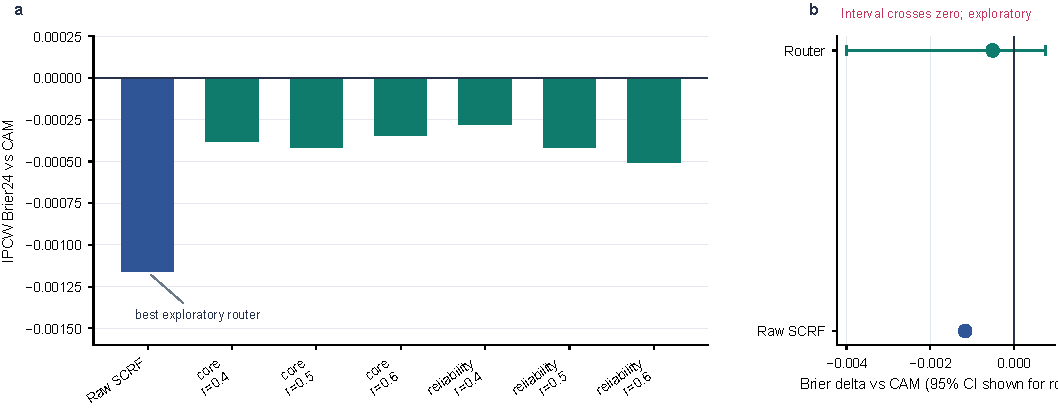
\includegraphics[width=\textwidth]{figures/extended_data_figure1_router_exploration.pdf}
\caption{\textbf{Exploratory patient-level reliability router.} \textbf{a}, IPCW Brier differences versus V0 for raw V1R and router policies. \textbf{b}, Best router point estimate with bootstrap interval. Reliability features improve routing relative to the core router and V0, while direct raw V1R remains the strongest full-coverage policy.}\label{fig:supp_router}
\end{figure*}

\clearpage
\section*{S15~Extension readouts: RADCURE, TCGA and GEO}
The RADCURE held-out analysis characterized adapted clinical/radiomics comparator families in 626 patients with 110 events. The strongest comparator, C2, achieved Uno C 0.806744, 24-month AUC 0.818182 and IPCW Brier 0.090683 (Table~\ref{tab:supptable5} and Fig.~\ref{fig:supp_radcure}). This analysis provides a strong contemporary benchmark for the multimodal prognostic task and highlights the value of combining clinical and tumour-volume information.

\begingroup
\scriptsize
\setlength{\tabcolsep}{3pt}
\begin{longtable}{lrrrrrr}
\caption{RADCURE held-out comparator characterization}\label{tab:supptable5}\\
\toprule
Comparator & Brier$_{24}$ & Uno C & AUC$_{24}$ & Harrell C & CITL & Calibration slope\\
\midrule
\endfirsthead
\multicolumn{7}{l}{\itshape Table S5 continued from previous page}\\
\toprule
Comparator & Brier$_{24}$ & Uno C & AUC$_{24}$ & Harrell C & CITL & Calibration slope\\
\midrule
\endhead
\bottomrule
\endlastfoot
C1 & 0.095801 & 0.806595 & 0.819376 & 0.795924 & $-0.097110$ & 1.950857\\
C2 & 0.090683 & 0.806744 & 0.818182 & 0.797862 & $-0.044444$ & 1.139466\\
C3 & 0.098469 & 0.771260 & 0.780742 & 0.761632 & $-0.099603$ & 1.268349\\
C4 & 0.097403 & 0.779243 & 0.787882 & 0.768812 & $-0.074520$ & 1.471544\\
\end{longtable}
\endgroup

\begin{figure*}[t]
\centering
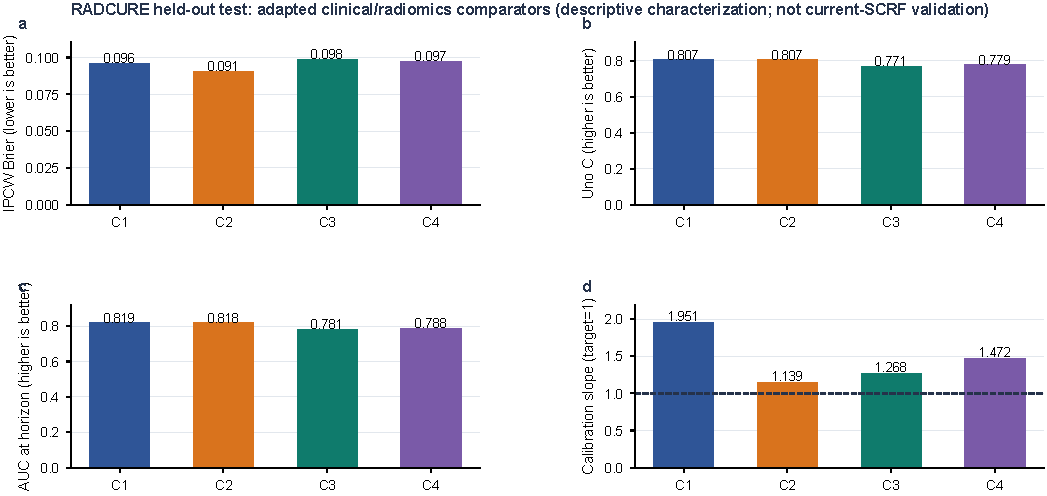
\includegraphics[width=\textwidth]{figures/extended_data_figure2_radcure_characterization.pdf}
\caption{\textbf{RADCURE characterization of adapted clinical/radiomics comparators.} \textbf{a--d}, IPCW Brier, Uno C, horizon AUC and calibration slope for C1--C4 in the held-out test split. C2 provides a strong benchmark by combining clinical predictors with tumour-volume information.}\label{fig:supp_radcure}
\end{figure*}

T1R improved every discrimination measure and the mean Brier score in TCGA-HNSC (Table~\ref{tab:supptable6}); discrimination improved in all five seeds (Table~\ref{tab:supptable7} and Fig.~\ref{fig:supp_t1r}). The frozen gate returned \texttt{T1R\_EARNS\_COMPLEXITY}. This demonstrates that the clinically anchored residual-shrinkage principle transfers to a dense transcriptome modality.

\begingroup
\scriptsize
\setlength{\tabcolsep}{2pt}
\begin{longtable}{>{\raggedright\arraybackslash}p{0.34\textwidth}rrrr}
\caption{T1R development performance in TCGA-HNSC}\label{tab:supptable6}\\
\toprule
Metric & Clinical anchor & T1R & Difference & Favourable seeds\\
\midrule
\endfirsthead
\multicolumn{5}{l}{\itshape Table S6 continued from previous page}\\
\toprule
Metric & Clinical anchor & T1R & Difference & Favourable seeds\\
\midrule
\endhead
\bottomrule
\endlastfoot
IPCW Brier at 24 months & 0.221795 & 0.218058 & $-0.003737$ & 4/5\\
Harrell C & 0.577281 & 0.605919 & $+0.028637$ & 5/5\\
Uno C at 24 months & 0.565199 & 0.597265 & $+0.032066$ & 5/5\\
Time-dependent AUC at 24 months & 0.557362 & 0.600236 & $+0.042874$ & 5/5\\
\end{longtable}
\endgroup

\begingroup
\scriptsize
\setlength{\tabcolsep}{3pt}
\begin{longtable}{lrr}
\caption{T1R paired changes by repetition seed}\label{tab:supptable7}\\
\toprule
Repetition seed & $\Delta$ IPCW Brier$_{24}$ & $\Delta$ Uno C$_{24}$\\
\midrule
\endfirsthead
\multicolumn{3}{l}{\itshape Table S7 continued from previous page}\\
\toprule
Repetition seed & $\Delta$ IPCW Brier$_{24}$ & $\Delta$ Uno C$_{24}$\\
\midrule
\endhead
\bottomrule
\endlastfoot
17 & $-0.004443$ & $+0.037975$\\
29 & $+0.002714$ & $+0.006398$\\
43 & $-0.004353$ & $+0.029370$\\
71 & $-0.006560$ & $+0.048165$\\
101 & $-0.006045$ & $+0.038420$\\
\end{longtable}
\endgroup

\begin{figure*}[t]
\centering
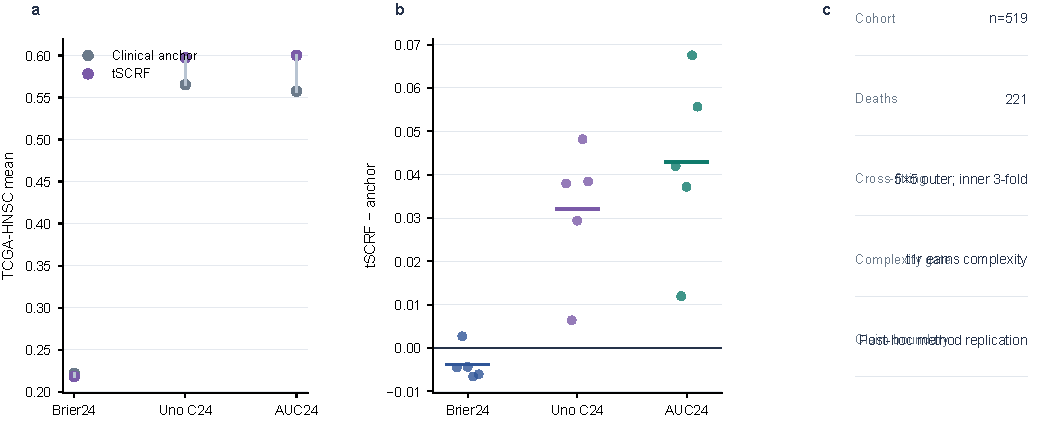
\includegraphics[width=\textwidth]{figures/extended_data_figure3_t1r_transcriptome_replication.pdf}
\caption{\textbf{T1R transcriptome method replication in TCGA-HNSC.} \textbf{a}, Mean anchor and T1R performance. \textbf{b}, Seed-level T1R$-$anchor differences. \textbf{c}, Cohort role and claim label. Discrimination improved in all five seeds.}\label{fig:supp_t1r}
\end{figure*}

A single T1R model fitted to the complete TCGA-HNSC development cohort showed favourable Brier and discrimination changes in both GEO cohorts (Table~\ref{tab:supptable8} and Fig.~\ref{fig:supp_geo}). In GSE65858, Uno C increased from 0.583694 to 0.645818. In GSE41613, the applied clinical anchor had no cross-patient variation, whereas T1R restored patient-level ordering, with Harrell C 0.626361 and 24-month AUC 0.634011. Calibration slopes above one indicate compressed predicted-risk dispersion, making cohort-level recalibration a constructive next step for prospective absolute-risk reporting.

\begingroup
\scriptsize
\setlength{\tabcolsep}{3pt}
\begin{longtable}{>{\raggedright\arraybackslash}p{0.31\textwidth}rrr}
\caption{GEO transcriptome characterization}\label{tab:supptable8}\\
\toprule
Cohort and metric & Clinical anchor & T1R & Difference\\
\midrule
\endfirsthead
\multicolumn{4}{l}{\itshape Table S8 continued from previous page}\\
\toprule
Cohort and metric & Clinical anchor & T1R & Difference\\
\midrule
\endhead
\bottomrule
\endlastfoot
\multicolumn{4}{l}{\textbf{GSE65858 (n=244; 78 events)}}\\
IPCW Brier at 24 months & 0.195207 & 0.195070 & $-0.000137$\\
Harrell C & 0.581806 & 0.644868 & $+0.063062$\\
Uno C at 24 months & 0.583694 & 0.645818 & $+0.062123$\\
Time-dependent AUC at 24 months & 0.588972 & 0.650733 & $+0.061762$\\
Calibration-in-the-large & $-0.763793$ & $-0.831959$ & $-0.068166$\\
Calibration slope & 1.707442 & 1.941562 & $+0.234120$\\
\multicolumn{4}{l}{\textbf{GSE41613 (n=97; 51 events)}}\\
IPCW Brier at 24 months & 0.265712 & 0.258607 & $-0.007104$\\
Harrell C & 0.500000 & 0.626361 & $+0.126361$\\
Uno C at 24 months & 0.500000 & 0.616039 & $+0.116039$\\
Time-dependent AUC at 24 months & 0.500000 & 0.634011 & $+0.134011$\\
Calibration-in-the-large & $-0.273717$ & $-0.264792$ & $+0.008925$\\
Calibration slope & -- & 1.939018 & --\\
\end{longtable}
\endgroup

\begin{figure*}[t]
\centering
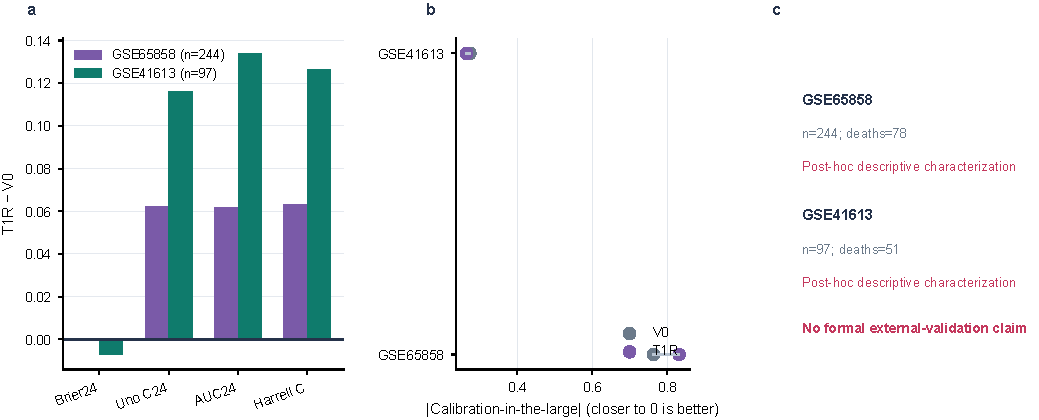
\includegraphics[width=\textwidth]{figures/extended_data_figure4_geo_t1r_characterization.pdf}
\caption{\textbf{GEO cross-platform characterization of T1R.} \textbf{a}, T1R$-$anchor differences in GSE65858 and GSE41613. \textbf{b}, Absolute calibration-in-the-large error. \textbf{c}, Cohort sizes and evidence role. A single frozen T1R fit retained favourable discrimination changes across platforms.}\label{fig:supp_geo}
\end{figure*}

\section*{S16~Reproducibility and artifact governance}
The formal V1R development out-of-fold SHA256 was \hashid{E43BB6C0D8E2C7F9C8B22A9C416AD752109B926A8526273D88811458CD73BCE0}. The confirmation protocol SHA256 was \hashid{1E134D30557D1CC153997F6EBB79E99C2E160F85A9F94BF3BBDD81C2C588BDED}, and the locked prediction artifact SHA256 was \hashid{E5DA83BDB3BB97C3488687C78CCF166FBD03059619DD0690E2767CAF8F393FCF}. Two V0 reruns produced identical out-of-fold hashes.

Aggregate sources included \path{U5R7_V1R_beta09_logloss_bridge_candidate/selected_bridge_aggregate_results.json}, \path{U6R1_patient_level_router_aggregation_exploration/u6r1_aggregate_results.json}, \path{U7R2_RADCURE_external_characterization/u7r2_radcure_external_characterization_aggregate_results.json}, \path{U8_T1R_transcriptome_residual_shrinkage/aggregate_t1r_transcriptome_development_cv_audit.json} and \path{U8E_T1R_external_characterization/aggregate_t1r_external_characterization_audit.json}, all under \path{research_studies/01_pattern_surv_hn/core_backbone/}. Figure provenance is recorded in \path{figures/figure_manifest.json}; publication figures are generated by \path{generate_figures.py}.

Cohorts, preprocessing and stage definitions were configuration controlled. Repetition seeds were 17, 29, 43, 71 and 101. Each stage recorded analysis label, prior outcome access, tuning status and artifact integrity. Patient identifiers and patient-level predictions were excluded from version control; publication-facing tables and figures were generated from aggregate metrics, manifests and audits. This governance allows every central number to be traced to a frozen artifact without redistributing restricted patient-level predictions.
